%! Licence = CC BY-NC-SA 4.0

%! Author = mariuszindel
%! Date = 30. Jan 2022
%! Project = Cheat-Sheet-Web-Engineering-3


\section{Firebase}

\subsection{Authentication}
\begin{itemize}
    \item Backend Services für Authentifizierung und einfache Userverwaltung
    \item SDKs für diverse Plattformen
    \item Vorgefertigte UI Libraries
\end{itemize}

\subsection{Hosting}
Einfaches Hosting für \textbf{statischen Content:}\\
immer HTTPS, Caching in CDN, Rollbacks\\
\textbf{Dynamischer Content:} nur über Cloud Functions oder Google App Engine (PaaS) oder Google Container / Kubernetes Engine (Docker)

\subsection{Cloud Functions}
Code als Reaktion auf einen Event ausführen (z.B.REST API) $\rightarrow$ AWS Lambda
%\begin{center}
%    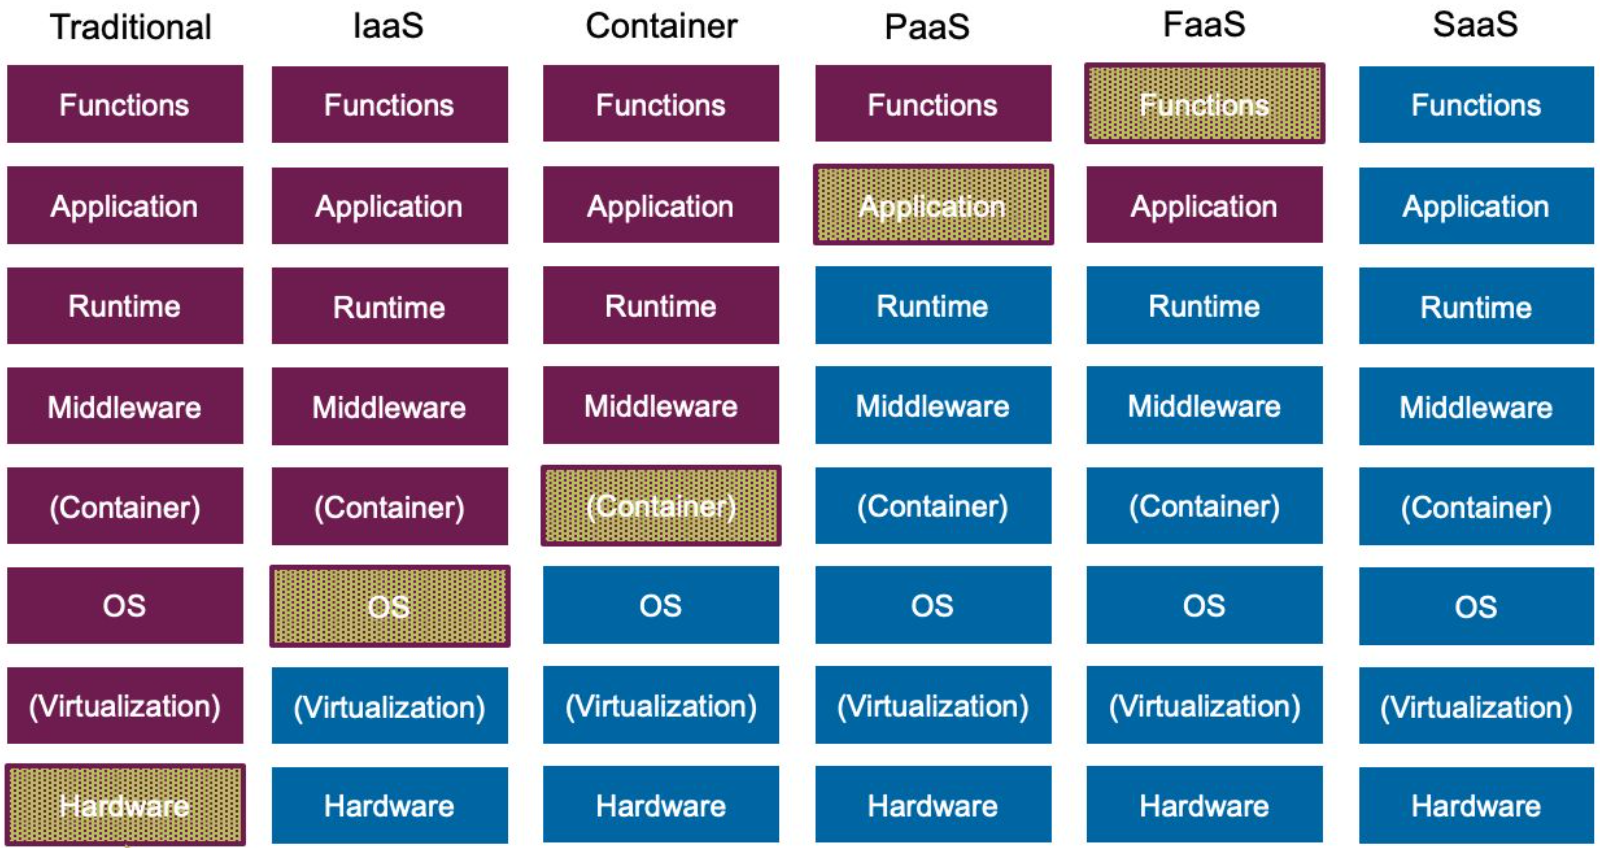
\includegraphics[width=1.0\linewidth]{./img/03-firebase/cloud_functions}
%    \vspace{-8pt}
%\end{center}

\subsubsection{Serverless Computing}
\textbf{Cloud Provider verwaltet Functions:}\\
Deployment on-demand, Plattform bestimmt Parallelisierung, Stateless Funktionen, Abgerechnet pro Aufruf / Laufzeit\\
\textbf{Limitationen:} Ausführungszeit \& Memory begrenzt, teilweise hohe Latenz.

\subsection{Cloud Firestore}
NoSQL, document-oriented database. DB aus mehreren Collections mit Dokumenten. Document ist JSON-Objekt. Document kann Collections beinhalten. Eingeschränkte Queries (keine Volltextsuche).

\subsubsection{NoSQL: Many-To-Many}
\begin{itemize}
    \item Wie in relationaler DB mit Assoziationstabelle
    \begin{itemize}[label={\textcolor{green}{+}}]
        \item Kein kopieren von Daten
    \end{itemize}
    \begin{itemize}[label={\textcolor{red}{--}}]
        \item Komplexere Abfragen, keine Joins in FS
    \end{itemize}
    \item Daten kopieren und einbetten
    \begin{itemize}[label={\textcolor{green}{+}}]
        \item Preisänderung eines Produktes hat keinen Einfluss auf vergangene Bestellungen.
    \end{itemize}
\end{itemize}
